\documentclass{article}
\usepackage{fontspec}
\usepackage{graphicx}
\usepackage{type1cm}
\usepackage{geometry}
\geometry{a4paper,left=1cm,right=1cm,top=3cm,bottom=3cm}
\usepackage[bold-style=ISO]{unicode-math}
% 添加heading=true, 使用中文版式
\usepackage[heading=true]{ctex}
% 生成pdf书签
\usepackage{hyperref}
% 自定义多级标题格式的宏包
\usepackage{titlesec} 
\titleformat{\section}[block]{\Huge\bfseries}{\arabic{section}}{1em}{}[]
\titleformat{\subsection}[block]{\huge\bfseries}{\arabic{section}.\arabic{subsection}}{1em}{}[]
\titleformat{\paragraph}[block]{\LARGE\bfseries}{[\arabic{paragraph}]}{1em}{}[]

\begin{document}
\begin{flushleft}
	\LARGE
	% \qquad 缩进两个字符
	
	\section{公式}

	\subsection{向量的模}
	
	设$\vec{a}=(x,y,z)$,则$|\vec{a}|=\sqrt{x^2+y^2+z^2}$\\
	~\\
	设$\alpha,\beta,\gamma$是向量$\vec{a}$与坐标轴的夹角,则$\vec{a}$的方向余弦分别为$cos\alpha=\frac{x}{\vec{a}},cos\beta=\frac{y}{\vec{a}},cos\gamma=\frac{z}{\vec{a}}$\\
	
	\subsection{向量的线性运算}
	
	1、$\vec{a}+\vec{b}=(a_x+b_x,a_y+b_y,a_z+b_z)$\\
	2、$\lambda\vec{a}=(\lambda a_x,\lambda a_y,\lambda a_z)$\\
	
	\subsection{向量的数量积}
	
	1、$\vec{a}\cdot\vec{b}=|\vec{a}||\vec{b}|cos\theta$,其中$\theta$是两个向量的夹角\\
	2、$\vec{a}\cdot\vec{b}=a_xb_x+a_yb_y+a_zb_z$\\
	3、两个向量垂直,即$\vec{a}\perp\vec{b}\Leftrightarrow\vec{a}\cdot\vec{b}=0$\\
	
	\subsection{向量的向量积}
	
	1、向量积的值:$|\vec{c}|=|\vec{a}\times\vec{b}|=|\vec{a}||\vec{b}|sin\theta$,其中$\theta$是两个向量的夹角\\
	2、向量积的方向:$\vec{c}$同时垂直于$\vec{a}$和$\vec{b}$\\
	3、行列式表示:$\vec{a}\times\vec{b}=
	\left|\begin{array}{cccc}
	\vec{i}&\vec{j}&\vec{k}\\
	a_x&a_y&a_z\\
	b_x&b_y&b_z
	\end{array}\right|$,其中$\vec{i},\vec{j},\vec{k}$是向量积在三个坐标轴上的分量\\
	4、两个向量平行,即$\vec{a}//\vec{b}\Leftrightarrow\vec{a}\times\vec{b}=0\Leftrightarrow\frac{a_x}{b_x}=\frac{a_y}{b_y}=\frac{a_z}{b_z}$\\
	
	\subsection{向量的混合积}
	
	1、$(\vec{a}\vec{b}\vec{c})=(\vec{a}\times\vec{b})\cdot\vec{c}=
	\left|\begin{array}{cccc}
	a_x&a_y&a_z\\
	b_x&b_y&b_z\\
	c_x&c_y&c_z
	\end{array}\right|$\\
	2、$\vec{a},\vec{b},\vec{c}$共面$\Leftrightarrow(\vec{a}\vec{b}\vec{c})=0$\\
	
	\subsection{平面的方程}
	
	\paragraph{平面的点法式方程}
	$A(x-x_0)+B(y-y_0)+C(z-z_0)=0$\\
	其中$(x_0,y_0,z_0)$为平面上的一个定点,$\vec{n}=(A,B,C)$为平面的法向量\\
	
	\paragraph{平面的一般式方程}
	$Ax+By+Cz+D=0$\\
	$\vec{n}=(A,B,C)$为法向量\\
	
	\paragraph{平面的截距式方程}
	$\frac{x}{a}+\frac{y}{b}+\frac{z}{c}=1$\\
	其中$a,b,c$分别为平面在三个坐标轴上的截距,且均不为$0$\\
	
	\subsection{空间直线的方程}
	
	\paragraph{空间直线的点向式方程}
	$\frac{x-x_0}{m}=\frac{y-y_0}{n}=\frac{z-z_0}{p}$\\
	其中$(x_0,y_0,z_0)$为直线上的一个定点,$\vec{s}=(m,n,p)$为直线的方向向量\\
	
	\paragraph{空间直线的参数式方程}
	$\left\{
	\begin{array}{lcl}
	x=x_0+mt\\
	y=y_0+nt\\
	z=z_0+pt
	\end{array} \right.$\\
	
	\paragraph{空间直线的一般式方程}
	$\left\{
	\begin{array}{lcl}
	A_1x+B_1y+C_1z+D_1=0\\
	A_2x+B_2y+C_2z+D_2=0
	\end{array} \right.$\\
	空间直线为两个平面的交线\\
	空间直线的方向向量为两个平面的法向量的向量积,即$\vec{s}=\vec{n_1}\times\vec{n_2}$\\
	
	\subsection{距离公式}
	
	1、点$P_1(x_1,y_1,z_1)$到点$P_2(x_2,y_2,z_2)$的距离\\$d=\sqrt{(x_2-x_1)^2+(y_2-y_1)^2+(z_2-z_1)^2}$\\~\\
	2、点$P_0(x_0,y_0,z_0)$到平面$Ax+By+Cz+D=0$的距离\\$d=\frac{|Ax_0+By_0+Cz_0+D|}{\sqrt{A^2+B^2+C^2}}$\\~\\
	3、点$P_0(x_0,y_0,z_0)$到空间直线$\frac{x-x_0}{m}=\frac{y-y_0}{n}=\frac{z-z_0}{p}$的距离\\$d=\frac{|\vec{P_0P}\times\vec{s}|}{|\vec{s}|}$\\
	\qquad 其中$P$是空间直线上的任意一点,\\
	\qquad $\vec{s}=(m,n,p)$为直线的方向向量\\
	
	\subsection{曲面的一般式}
	$F(x,y,z)=0$\\
	
	\subsection{旋转曲面方程}
	
	\paragraph{旋转曲面}
	旋转曲面是一条平面曲线绕着它所在的平面上一条固定直线旋转一周所生成的曲面。该固定直线称为旋转轴,该旋转曲线称为母线。
	
	\paragraph{建立旋转曲面方程}
	设$yOz$坐标面上有一条曲线$L=\left\{
	\begin{array}{lcl}
	f(y,z)=0\\
	x=0
	\end{array} \right.$,\\
	该曲线绕$z$轴旋转一周的方程为:$f(\pm\sqrt{x^2+y^2},z)=0$\\
	该曲线绕$y$轴旋转一周的方程为:$f(\pm\sqrt{y,x^2+z^2})=0$\\
	
	\subsection{柱面方程}
	
	\paragraph{柱面}
	柱面是直线沿着一条定曲线平行移动所形成的曲面,即动直线沿着一条定曲线平行移动所形成的曲面,动直线称为柱面的直母线,定曲线称为柱面的准线。
	
	\paragraph{建立柱面方程}
	缺一个字母的曲面方程就是柱面方程,如方程$F(x,y)=0$表示一个母线平行于$z$轴的柱面\\
	
	\subsection{二次曲面}
	
	\paragraph{圆锥面}
	$z^2=a(x^2+y^2)$\\
	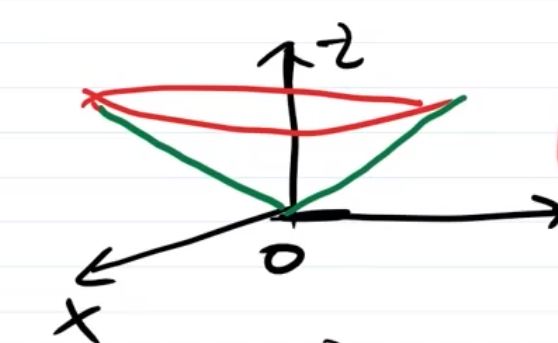
\includegraphics[scale=0.5]{yzm.png}
	
	\paragraph{抛物面}
	$z=a(x^2+y^2)$\\
	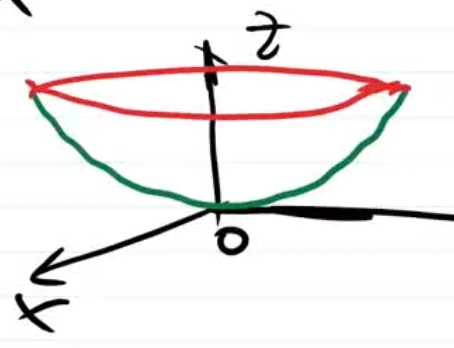
\includegraphics[scale=0.5]{pwm.png}
	
	\paragraph{椭球}
	$\frac{x^2}{a^2}+\frac{y^2}{b^2}+\frac{z^2}{c^2}=1$\\
	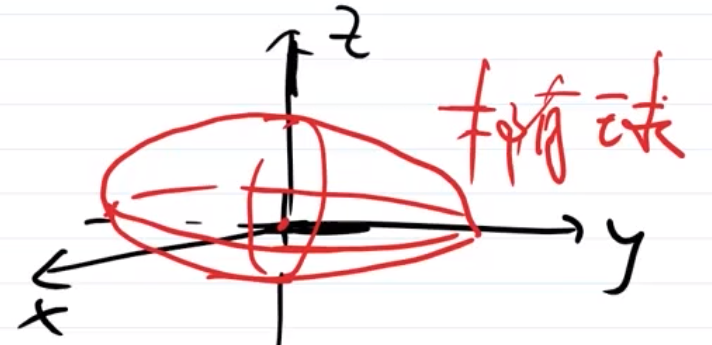
\includegraphics[scale=0.5]{tq.png}
	
	\paragraph{圆柱面}
	$x^2+y^2=R^2$\\
	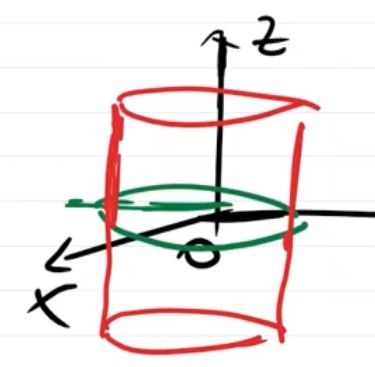
\includegraphics[scale=0.5]{yz.png}
	
	\paragraph{单叶双曲面}
	$\frac{x^2}{a^2}+\frac{y^2}{b^2}-\frac{z^2}{c^2}=1$\\
	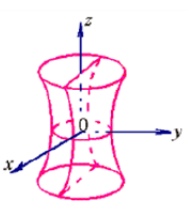
\includegraphics[scale=0.5]{dysqm.png}
	
	\paragraph{双叶双曲面}
	$\frac{x^2}{a^2}+\frac{y^2}{b^2}-\frac{z^2}{c^2}=-1$\\
	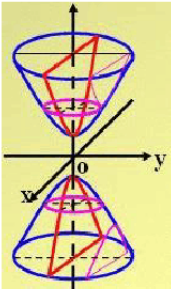
\includegraphics[scale=0.5]{sysqm.png}
	
	\subsection{空间曲线的方程}
	
	\paragraph{一般式}
	$\left\{
	\begin{array}{lcl}
	F(x,y,z)=0\\
	G(x,y,z)=0
	\end{array} \right.$\\
	
	\paragraph{参数式}
	$\left\{
	\begin{array}{lcl}
	x=x(t)\\
	y=y(t)\\
	z=z(t)
	\end{array} \right.$\\
	
	\paragraph{空间曲线在坐标面上的投影}
	设空间曲线$C=\left\{
	\begin{array}{lcl}
	F(x,y,z)=0\\
	G(x,y,z)=0
	\end{array} \right.$,\\
	在此方程组中消去$z$,得到$H(x,y)=0$,它表示空间曲线$C$关于$xOy$面的投影柱面。\\
	若令$z=0$,则$\left\{
	\begin{array}{lcl}
	H(x,y)=0\\
	z=0
	\end{array} \right.$表示空间曲线$C$在$xOy$面上的投影\\
	
	
	
\end{flushleft}
\end{document}